\documentclass{standalone}
\usepackage{tikz}
\usetikzlibrary{patterns, positioning}

\begin{document}
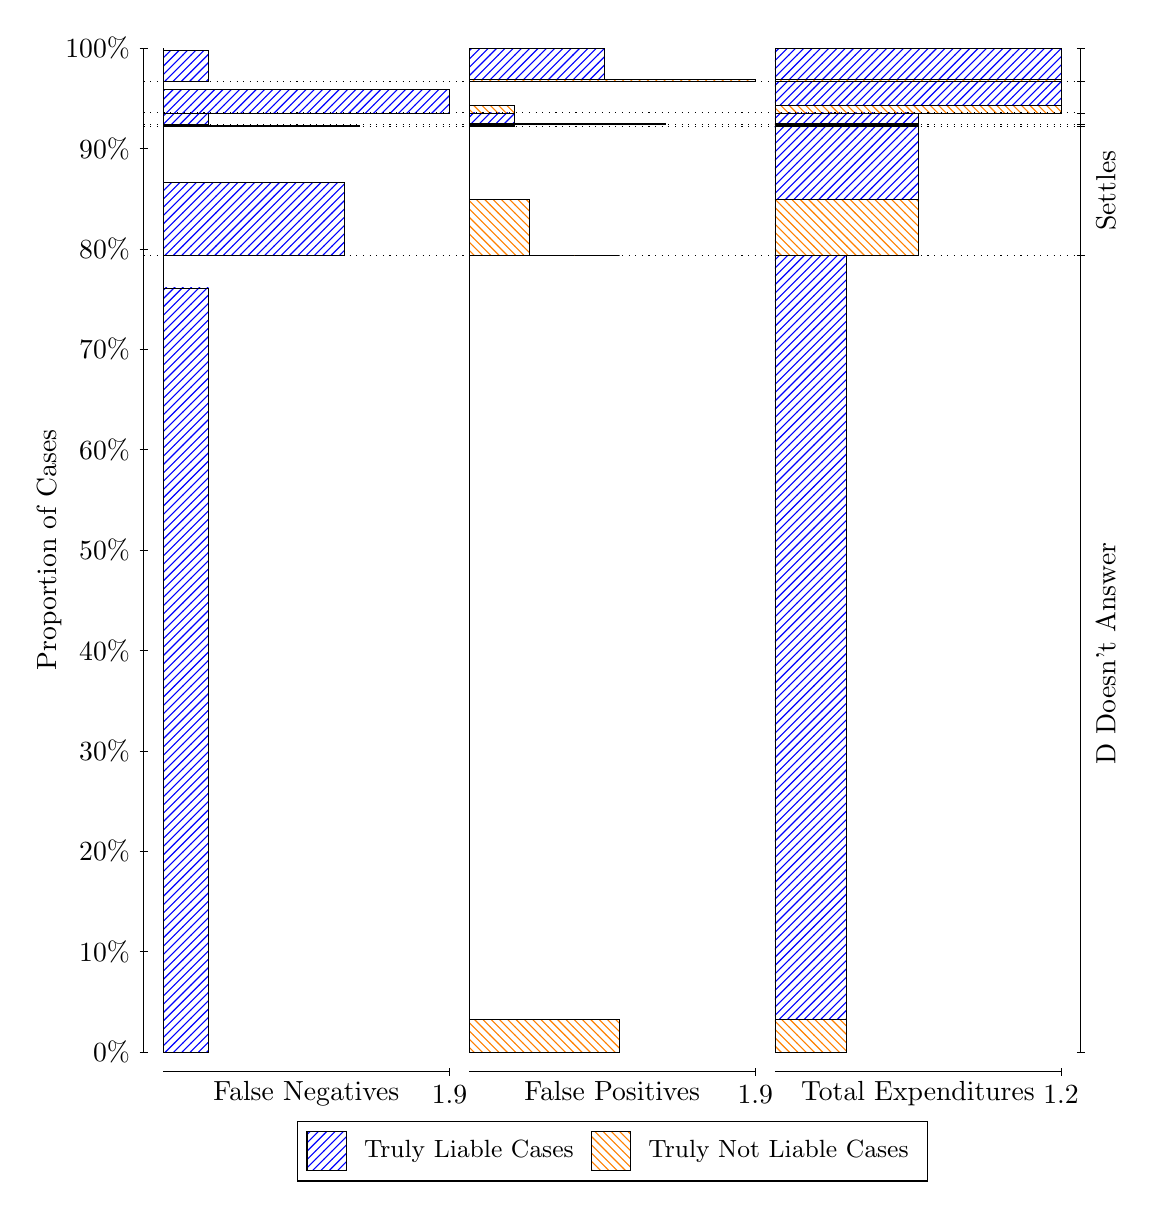
\begin{tikzpicture}
\draw[black, very thin] (1.5,1.75) -- (1.5,14.5);
\node[rotate=90, anchor=center] at (0.3, 8.125) {Proportion of Cases};
\draw[black, very thin] (1.45,1.75) -- (1.55,1.75);
\node[anchor=east] at (1.45, 1.75) {0\%};
\draw[black, very thin] (1.45,3.025) -- (1.55,3.025);
\node[anchor=east] at (1.45, 3.025) {10\%};
\draw[black, very thin] (1.45,4.3) -- (1.55,4.3);
\node[anchor=east] at (1.45, 4.3) {20\%};
\draw[black, very thin] (1.45,5.575) -- (1.55,5.575);
\node[anchor=east] at (1.45, 5.575) {30\%};
\draw[black, very thin] (1.45,6.85) -- (1.55,6.85);
\node[anchor=east] at (1.45, 6.85) {40\%};
\draw[black, very thin] (1.45,8.125) -- (1.55,8.125);
\node[anchor=east] at (1.45, 8.125) {50\%};
\draw[black, very thin] (1.45,9.4) -- (1.55,9.4);
\node[anchor=east] at (1.45, 9.4) {60\%};
\draw[black, very thin] (1.45,10.675) -- (1.55,10.675);
\node[anchor=east] at (1.45, 10.675) {70\%};
\draw[black, very thin] (1.45,11.95) -- (1.55,11.95);
\node[anchor=east] at (1.45, 11.95) {80\%};
\draw[black, very thin] (1.45,13.225) -- (1.55,13.225);
\node[anchor=east] at (1.45, 13.225) {90\%};
\draw[black, very thin] (1.45,14.5) -- (1.55,14.5);
\node[anchor=east] at (1.45, 14.5) {100\%};

\draw[black, very thin] (13.4,1.75) -- (13.4,14.5);
\draw[black, very thin] (13.35,1.75) -- (13.45,1.75);
\node[anchor=west] at (13.35, 1.75) {};
\draw[black, very thin] (13.35,11.867) -- (13.45,11.867);
\node[anchor=west] at (13.35, 11.867) {};
\draw[black, very thin] (13.35,13.509) -- (13.45,13.509);
\node[anchor=west] at (13.35, 13.509) {};
\draw[black, very thin] (13.35,13.531) -- (13.45,13.531);
\node[anchor=west] at (13.35, 13.531) {};
\draw[black, very thin] (13.35,13.676) -- (13.45,13.676);
\node[anchor=west] at (13.35, 13.676) {};
\draw[black, very thin] (13.35,14.072) -- (13.45,14.072);
\node[anchor=west] at (13.35, 14.072) {};
\draw[black, very thin] (13.35,14.5) -- (13.45,14.5);
\node[anchor=west] at (13.35, 14.5) {};

\draw[black, very thin, pattern color=blue, pattern=north east lines] (1.75,1.75) rectangle (2.3237,11.455);
\draw[black, very thin, pattern color=orange, pattern=north west lines] (1.75,11.455) rectangle (1.75,11.867);
\draw[black, very thin, pattern color=blue, pattern=north east lines] (1.75,11.867) rectangle (4.0447,12.797);
\draw[black, very thin, pattern color=blue, pattern=north east lines] (1.75,12.797) rectangle (3.8535,12.797);
\draw[black, very thin, pattern color=blue, pattern=north east lines] (1.75,12.797) rectangle (3.6623,12.797);
\draw[black, very thin, pattern color=blue, pattern=north east lines] (1.75,12.797) rectangle (3.4711,12.797);
\draw[black, very thin, pattern color=blue, pattern=north east lines] (1.75,12.797) rectangle (3.4711,12.797);
\draw[black, very thin, pattern color=blue, pattern=north east lines] (1.75,12.797) rectangle (3.2798,12.797);
\draw[black, very thin, pattern color=blue, pattern=north east lines] (1.75,12.797) rectangle (3.0886,12.797);
\draw[black, very thin, pattern color=blue, pattern=north east lines] (1.75,12.797) rectangle (2.8974,12.797);
\draw[black, very thin, pattern color=orange, pattern=north west lines] (1.75,12.797) rectangle (1.75,13.509);
\draw[black, very thin, pattern color=blue, pattern=north east lines] (1.75,13.509) rectangle (4.236,13.519);
\draw[black, very thin, pattern color=orange, pattern=north west lines] (1.75,13.519) rectangle (1.75,13.531);
\draw[black, very thin, pattern color=blue, pattern=north east lines] (1.75,13.531) rectangle (2.3237,13.668);
\draw[black, very thin, pattern color=orange, pattern=north west lines] (1.75,13.668) rectangle (1.75,13.676);
\draw[black, very thin, pattern color=blue, pattern=north east lines] (1.75,13.676) rectangle (5.3833,13.974);
\draw[black, very thin, pattern color=orange, pattern=north west lines] (1.75,13.974) rectangle (1.75,14.072);
\draw[black, very thin, pattern color=blue, pattern=north east lines] (1.75,14.072) rectangle (2.3237,14.467);
\draw[black, very thin, pattern color=orange, pattern=north west lines] (1.75,14.467) rectangle (1.75,14.5);
\draw[black, very thin, pattern color=orange, pattern=north west lines] (5.6333,1.75) rectangle (7.5456,2.1621);
\draw[black, very thin, pattern color=blue, pattern=north east lines] (5.6333,2.1621) rectangle (5.6333,11.867);
\draw[black, very thin, pattern color=orange, pattern=north west lines] (5.6333,11.867) rectangle (7.5456,11.867);
\draw[black, very thin, pattern color=orange, pattern=north west lines] (5.6333,11.867) rectangle (7.3544,11.867);
\draw[black, very thin, pattern color=orange, pattern=north west lines] (5.6333,11.867) rectangle (7.1632,11.867);
\draw[black, very thin, pattern color=orange, pattern=north west lines] (5.6333,11.867) rectangle (6.9719,11.867);
\draw[black, very thin, pattern color=orange, pattern=north west lines] (5.6333,11.867) rectangle (6.7807,11.867);
\draw[black, very thin, pattern color=orange, pattern=north west lines] (5.6333,11.867) rectangle (6.5895,11.867);
\draw[black, very thin, pattern color=orange, pattern=north west lines] (5.6333,11.867) rectangle (6.3982,12.579);
\draw[black, very thin, pattern color=blue, pattern=north east lines] (5.6333,12.579) rectangle (5.6333,13.509);
\draw[black, very thin, pattern color=orange, pattern=north west lines] (5.6333,13.509) rectangle (6.207,13.521);
\draw[black, very thin, pattern color=blue, pattern=north east lines] (5.6333,13.521) rectangle (5.6333,13.531);
\draw[black, very thin, pattern color=orange, pattern=north west lines] (5.6333,13.531) rectangle (8.1193,13.539);
\draw[black, very thin, pattern color=blue, pattern=north east lines] (5.6333,13.539) rectangle (6.207,13.676);
\draw[black, very thin, pattern color=orange, pattern=north west lines] (5.6333,13.676) rectangle (6.207,13.774);
\draw[black, very thin, pattern color=blue, pattern=north east lines] (5.6333,13.774) rectangle (5.6333,14.072);
\draw[black, very thin, pattern color=orange, pattern=north west lines] (5.6333,14.072) rectangle (9.2667,14.105);
\draw[black, very thin, pattern color=blue, pattern=north east lines] (5.6333,14.105) rectangle (7.3544,14.5);
\draw[black, very thin, pattern color=orange, pattern=north west lines] (9.5167,1.75) rectangle (10.425,2.1621);
\draw[black, very thin, pattern color=blue, pattern=north east lines] (9.5167,2.1621) rectangle (10.425,11.867);
\draw[black, very thin, pattern color=orange, pattern=north west lines] (9.5167,11.867) rectangle (11.333,11.867);
\draw[black, very thin, pattern color=blue, pattern=north east lines] (9.5167,11.867) rectangle (11.333,11.867);
\draw[black, very thin, pattern color=orange, pattern=north west lines] (9.5167,11.867) rectangle (11.333,12.579);
\draw[black, very thin, pattern color=blue, pattern=north east lines] (9.5167,12.579) rectangle (11.333,13.509);
\draw[black, very thin, pattern color=orange, pattern=north west lines] (9.5167,13.509) rectangle (11.333,13.509);
\draw[black, very thin, pattern color=blue, pattern=north east lines] (9.5167,13.509) rectangle (11.333,13.509);
\draw[black, very thin, pattern color=orange, pattern=north west lines] (9.5167,13.509) rectangle (11.333,13.521);
\draw[black, very thin, pattern color=blue, pattern=north east lines] (9.5167,13.521) rectangle (11.333,13.531);
\draw[black, very thin, pattern color=orange, pattern=north west lines] (9.5167,13.531) rectangle (11.333,13.539);
\draw[black, very thin, pattern color=blue, pattern=north east lines] (9.5167,13.539) rectangle (11.333,13.676);
\draw[black, very thin, pattern color=orange, pattern=north west lines] (9.5167,13.676) rectangle (13.15,13.774);
\draw[black, very thin, pattern color=blue, pattern=north east lines] (9.5167,13.774) rectangle (13.15,14.072);
\draw[black, very thin, pattern color=orange, pattern=north west lines] (9.5167,14.072) rectangle (13.15,14.105);
\draw[black, very thin, pattern color=blue, pattern=north east lines] (9.5167,14.105) rectangle (13.15,14.5);
\draw[black, dotted] (1.5,11.867) -- (13.4,11.867);
\draw[black, dotted] (1.5,13.509) -- (13.4,13.509);
\draw[black, dotted] (1.5,13.531) -- (13.4,13.531);
\draw[black, dotted] (1.5,13.676) -- (13.4,13.676);
\draw[black, dotted] (1.5,14.072) -- (13.4,14.072);
\draw[black, very thin] (1.75,1.5) -- (5.3833,1.5);
\node[anchor=north] at (3.5667, 1.5) {False Negatives};
\draw[black, very thin] (5.3833,1.45) -- (5.3833,1.55);
\node[anchor=north] at (5.3833, 1.45) {1.9};

\draw[black, very thin] (5.6333,1.5) -- (9.2667,1.5);
\node[anchor=north] at (7.45, 1.5) {False Positives};
\draw[black, very thin] (9.2667,1.45) -- (9.2667,1.55);
\node[anchor=north] at (9.2667, 1.45) {1.9};

\draw[black, very thin] (9.5167,1.5) -- (13.15,1.5);
\node[anchor=north] at (11.333, 1.5) {Total Expenditures};
\draw[black, very thin] (13.15,1.45) -- (13.15,1.55);
\node[anchor=north] at (13.15, 1.45) {1.2};

\node[black, centered, rotate=90] at (13.72, 6.8087) {D Doesn't Answer};
\node[black, centered, rotate=90] at (13.72, 12.688) {Settles};





\draw (7.449999999999999,1.5) node[draw=none] (baseCoordinate) {};
\begin{scope}[align=center]
        \matrix[scale=0.5, draw=black, below=0.5cm of baseCoordinate, nodes={draw}, column sep=0.1cm]{
            \node[rectangle, draw, minimum width=0.5cm, minimum height=0.5cm, pattern=north east lines, pattern color=blue] {}; &
            \node[draw=none, font=\small] (B) {Truly Liable Cases}; &
            \node[rectangle, draw, minimum width=0.5cm, minimum height=0.5cm, pattern=north west lines, pattern color=orange] {}; &
            \node[draw=none, font=\small] (B) {Truly Not Liable Cases}; \\
            };
\end{scope}

\end{tikzpicture}
\end{document}